% ****** Start of file apssamp.tex ******
%
%   This file is part of the APS files in the REVTeX 4.1 distribution.
%   Version 4.1r of REVTeX, August 2010
%
%   Copyright (c) 2009, 2010 The American Physical Society.
%
%   See the REVTeX 4 README file for restrictions and more information.
%
% TeX'ing this file requires that you have AMS-LaTeX 2.0 installed
% as well as the rest of the prerequisites for REVTeX 4.1
%
% See the REVTeX 4 README file
% It also requires running BibTeX. The commands are as follows:
%
%  1)  latex apssamp.tex
%  2)  bibtex apssamp
%  3)  latex apssamp.tex
%  4)  latex apssamp.tex
%
\documentclass[%
% reprint,
%superscriptaddress,
%groupedaddress,
%unsortedaddress,
%runinaddress,
%frontmatterverbose, 
preprint,
%showpacs,preprintnumbers,
%nofootinbib,
%nobibnotes,
bibnotes,
% amsmath,amssymb,
% aps,
%pra,
%prb,	
%rmp,
%prstab,
%prstper,
%floatfix,
]{revtex4-1}

\usepackage{graphicx}% Include figure files
\usepackage{dcolumn}% Align table columns on decimal point
\usepackage{bm}% bold math
%\usepackage{hyperref}% add hypertext capabilities
%\usepackage[mathlines]{lineno}% Enable numbering of text and display math
%\linenumbers\relax % Commence numbering lines

%\usepackage[showframe,%Uncomment any one of the following lines to test 
%%scale=0.7, marginratio={1:1, 2:3}, ignoreall,% default settings
%%text={7in,10in},centering,
%%margin=1.5in,
%%total={6.5in,8.75in}, top=1.2in, left=0.9in, includefoot,
%%height=10in,a5paper,hmargin={3cm,0.8in},
%]{geometry}

\begin{document}

%\preprint{APS/123-QED}
%\begin{titlepage}
\includegraphics[width= 40mm]{aleph-logo.jpg}
\title{Proposal for Two-Particle Correlation Analyses with ALEPH Data}% Force line breaks with \\
%\thanks{A footnote to the article title}%

\author{Bibek Pandit}%
 \email{bibek@mit.edu}
\author{Anthony Badea}%
 \email{badea@mit.edu}
\author{Gian Michele Innocenti}%
 \email{ginnocen@mit.edu }
\author{Yen-Jie Lee}
 \email{yenjie@mit.edu}
 \affiliation{Massachusetts Institute of Technology}%
% \altaffiliation[Also at ]{Physics Department, XYZ University.}%Lines break automatically or can be forced with \\

%\collaboration{BELLE Collaboration}%\noaffiliation

\date{\today}% It is always \today, today,
             %  but any date may be explicitly specified

\begin{abstract}
Two-particle correlations in high-energy collisions provide valuable information for characterizing Quantum Chromodynamics and have been studied previously for a broad range of collision energies in proton-proton (pp), proton-nucleus (pA), and nucleus-nucleus (AA) collisions. In AA collisions, a significant long-range angular correlation between particles was observed. The common interpretation of the results based on the hydrodynamics calculations was that a thermalized system was created in the AA collisions. Recently, similar correlation signals were observed in high particle multiplicity pp and pA collisions. The physical origin of the phenomenon is not yet fully understood. Due to the complexity of the hadron-hadron collisions, possible initial state correlations of the partons, such as those arise from color-glass condensate, could complicate the interpretation of the pp and pA data. Studies of high multiplicity $e^+e^-$ collision, where the initial kinematics of the collisions are well-controlled, could bring significant insights about the observed phenomenon. This paper proposes measurements of two-particle angular correlations of charged hadrons produced in $e^+e^-$ collisions, as a function of charged hadron multiplicity with the ALEPH detector. These measurements will enable a direct comparison between $e^+e^-$, pp, pA and AA collisions for the first time. Preliminary results from Belle open data are also presented.
\end{abstract}

\pacs{Valid PACS appear here}% PACS, the Physics and Astronomy
                             % Classification Scheme.
%\keywords{Suggested keywords}%Use showkeys class option if keyword
                              %display desired
\maketitle

%\tableofcontents

%%% Introduction %%%
\section{Introduction}

This analysis note presents the measurements of two-particle angular correlations of charged hadrons produced in $e^+e^-$ collisions as a function of charged hadron multiplicity, using 730 $pb^{-1}$ of archived data collected between 91 and 209 GeV with the ALEPH detector at LEP.  Two-particle correlations in high-energy collisions provide valuable information for characterizing Quantum Chromodynamics and have been studied previously for a broad range of collision energies in proton-proton (pp)~\cite{Khachatryan:2010gv}, proton-nucleus (pA)~\cite{CMS:2012qk,Abelev:2012ola,Aad:2012gla}, and nucleus-nucleus (AA)~\cite{Aamodt:2010pa,Chatrchyan:2012wg} collisions. Such measurements can elucidate the underlying mechanism of particle production and reveal possible collective effects resulting from the high particle densities accessible in these collisions.

Studies of two-particle angular correlations in pp, pA and AA collisions are typically performed using two-dimensional $\Delta\eta-\Delta\phi$ correlation functions, where $\Delta\phi$ is the difference in the azimuthal angle $\phi$ between the two particles and $\Delta\eta$ is the difference in pseudorapidity $\eta = -\ln(\tan(\theta/2))$. The polar angle $\theta$ is defined relative to the counterclockwise hadron beam direction.

Of particular interest in studies of collective effects is the long-range (large $|\Delta\eta|$) structure of the two-particle correlation functions. In this region, the function is less susceptible to other known sources of correlations such as resonance decays and fragmentation function of energetic jets. Measurements in high-energy AA collisions have shown significant modification of the long-range structure compared with minimum-bias pp collisions, over a very wide range of collision energies~\cite{Back:2004je,Arsene:2004fa,Adcox:2004mh,Adams:2005dq}. The long-range correlations are commonly interpreted as a consequence of the hydrodynamical flow of the produced strongly interacting medium~\cite{Ollitrault:1992bk} and usually characterized by the Fourier components of the azimuthal particle distributions. The extraction of the second and third Fourier components, usually referred to as elliptic and triangular flow, is of great interest because it is closely related to initial collision geometry and its fluctuation~\cite{Alver:2010gr}. Those measurements allow the extraction of the fundamental transport properties of the medium using hydrodynamic models.

Recently, measurements in pp~\cite{Khachatryan:2010gv} and pPb collisions~\cite{CMS:2012qk,Abelev:2012ola,Aad:2012gla} have revealed the emergence of long-range, near-side ($\Delta\phi\sim 0$) correlations in the selection of collisions with very high number of final state particles. This ``ridge-like'' correlation has inspired a large variety of theoretical models~\cite{Bzdak:2013zma,Dusling:2015gta}. The physical origin of the phenomenon is not yet fully understood. Moreover, it was found that the elliptic flow signal exists even at the lowest nucleon-nucleon center-of-mass energy of 7.7 GeV in AA collisions at the Relativistic Heavy Ion Collider~\cite{Adamczyk:2012ku}. 

Due to the complexity of the hadron-hadron collisions, possible initial state correlations of the partons, such as those arise from color-glass condensate~\cite{Gelis:2010nm, Dusling:2013qoz}, could complicate the interpretation of the pp and pA data. Studies of high multiplicity $e^+e^-$ collision, where the initial kinematics of the collisions are well-controlled, could bring significant insights about the observed phenomenon. These measurements will also enable a direct comparison between different collision systems for the first time. The studies of ridge signal in $e^+e^-$ collisions will bring significant impact to the field of relativistic heavy ion collisions, either change completely the interpretation of the ridge in pp, pA and AA collisions if a significant signal is observed, or serve as an important reference for the final state effect observed in high multiplicity hadron-hadron scatterings if no long-range correlation signal was detected. 

With the archived data from ALEPH collaboration, the correlation functions are studied over a broad range of pseudorapidity $\eta$ (rapidity $y$) and azimuthal angle $\phi$ with respect to the electron-positron beam axis. In addition, the correlation functions are also studied using azimuthal and polar angles calculated with respect to the the event thrust axis and a dijet axis in order to follow the direction of the extending color strings. 


%%% Data %%%
\section{Data Sample}

The ALEPH archieved data used in this analysis will be documented in this section, which include both LEP1 and LEP2 period.



%%% Analysis %%%
\section{Analysis}

%Thrust Axis Reconstruction
\section{Thrust and sphericity axes}

The thrust $T$, and the thrust axis, $\hat{n}$, are defined as using the vector which maximizes the sum of the projection of the momenta of all particles in the event onto the axis:

\begin{equation}
T = max_{\hat{n}} \frac {\sum_i \left| \hat{p}_i . \hat{n} \right|}{\sum_i \left| \hat{p}_i \right|}.
\end{equation}

Events which are 'pencil-like' in shape are expected to have $T$ close to unity, while events in which the particles are distributed rather isotropically are expected to have $T$ close to 0.5.  

The thrust is calculated for an event having $n$ particles, each having a momentum $\vec{p_{i}}$, using an iterative procedure. The initial thrust axis, $\vec{T_0}$ is first taken to be a unit vector along the axis of any particle.  The thrust axis is then updated according to

\begin{equation}
\vec{T}_{i+1} = \vec{T}_{i}+\sum\limits_{j=1}^n  \rm{sign}(\vec{p_j}\cdot\vec{T}_i)\vec{p_{j}}.
\end{equation}

This procedure is repeated until there have either been $n$ iterations, or when the sign of $\vec{p_j}\cdot\vec{T_i}$ does not change for every particle between the $i$ and $i+1$ iterations.  The resulting vector, $\vec{T}_{\rm{cand}}$, is then stored as a thrust axis candidate.  The entire procedure is then repeated $n$ times, each time starting with a new initial particle, to give $n$ thrust axis candidates.  The candidate which maximizes the quantity $T$ is then chosen as the final thrust axis.

Another event shape variable used in this analysis is the sphericity axis.  The sphericity tensor is defined as
\begin{equation}
S^{\alpha\beta}=\frac{\sum\limits_{i}p_{i}^{\alpha}p_{i}^{\beta}}{\sum\limits_{i}|p_{i}|^2},
\end{equation}
where $\alpha$ and $\beta$ can take on values of one to three, corresponding to the $x$, $y$, and $z$ axes.  This can be diagonalized and three eigenvalues, $\lambda_{1}\geq\lambda_{2}\geq\lambda_{3}$ can be found, whose sum is unity.  The sphericity is defined as

\begin{equation}
S=\frac{3}{2}(\lambda_{2}+\lambda_{3}).
\end{equation}
It is bound between zero and one, with zero corresponding to a 'pencil-like' event and one corresponding to an isotropic event.  A related variable, the Aplanarity is defined as

\begin{equation}
A=\frac{3}{2}(\lambda_{3}).
\end{equation}
A planar event has $A=0$, while an isotropic one has $A=0.5$.

The sphericity axis, $\vec{S}$ is simply defined as the eigenvector corresponding to $\lambda_1$.

%Reproduce QCD paper plots
\section{Thrust distribution}

In order to validate the ALEPH archived data sample and our understanding,
an analysis of the thrust distribution ($T$) is performed with LEP1 archived
data. The distributions are corrected for the detector response by ALEPH MC
produced in 1994. The results are unfolded by a Bayesian unfolding method. The size of the correction factor is small in the mid-$T$
and becomes larger as we go to smaller $T$ or larger $T$ regions.

%\begin{figure}[H]
%\centering
%\includegraphics[width=.5\textwidth]{images/Thrust/correction.pdf}
%\caption{The correction factor for the Thrust distribution measurement obtained from ALEPH MC.}
%\label{fig:ThrustCorr}
%\end{figure}

Figure~\ref{fig:ThrustResults} shows the corrected thrust distribution from ALEPH archived data. The results are compared to ALEPH
publications~\cite{Barate:1996fi,heister:2003aj}. As shown in the figure, a very good agreement between ALEPH archived data from this note
and ALEPH publications in the low $T$ region. In the $T\sim 1$ region, a small difference at the level of 0-10\% is observed between this work
and the ALEPH publication in 2004~\cite{heister:2003aj}. This could be due to the difference in unfolding procedure, the dataset used and the event selection criteria.


\begin{figure}[H]
\centering
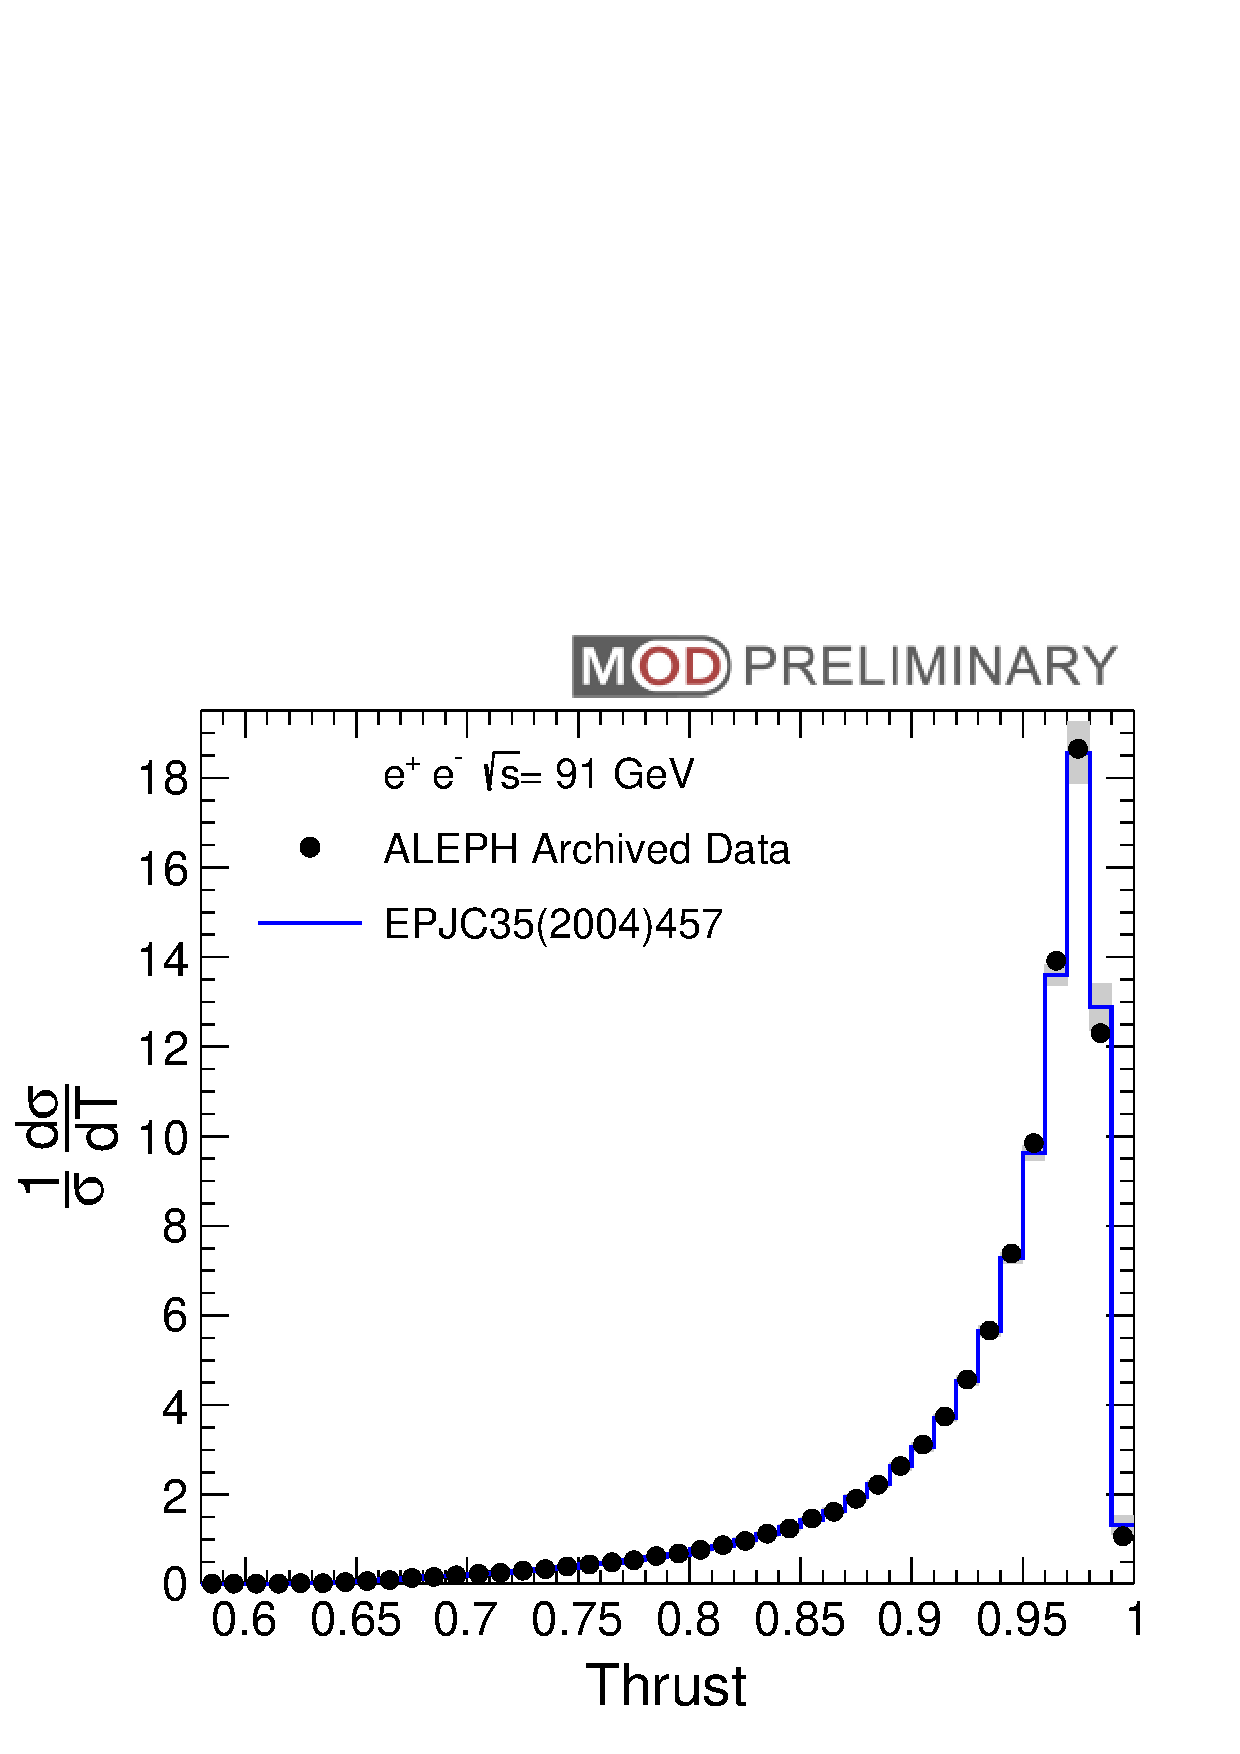
\includegraphics[width=.49\textwidth]{images/Thrust/ThrustResult.png}
\includegraphics[width=.49\textwidth]{images/Thrust/ThrustResultLogY.png}
\caption{The corrected thrust distribution from ALEPH archived data compared to previous publications in linear and log scale.}
\label{fig:ThrustResults}
\end{figure}


%Two Particle Correlation Analysis
\section{Two-Particle Correlation Function}
\makeatletter
\DeclareRobustCommand{\textsupsub}[2]{{%
  \m@th\ensuremath{%
    ^{\mbox{\fontsize\sf@size\z@#1}}%
    _{\mbox{\fontsize\sf@size\z@#2}}%
  }%
}}
\makeatother

In this analysis with ALEPH open data, charged particles with transverse momentum between 0.1 and 4.0 GeV/$c$ 
are selected for the correlation function analysis. High multiplicity events are sampled using the total number of selected proton, 
pions and kaons (hadron multiplicity $N$) in each event. The first step in extracting the correlation function was to divide the sample 
into bins in the hadron multiplicity. For each hadron multiplicity class, ``trigger" particles are defined as charged hadrons in the selected transverse momentum range (0.1 and 4.0 GeV/$c$). Particle pairs are then formed by associating every trigger particle with the remaining charged hadrons in the same $p_{\rm T}$ interval as the trigger particle. The per-trigger-particle associated yield is defined as:
\begin{eqnarray}
\label{eq:associatedyield}
\frac{1}{N_{\rm trig}}\frac{\rm d^2N^{pair}}{d\Delta\eta  \rm d\Delta\phi}= B(0,0) \times \frac{S(\Delta\eta, \Delta\phi)}{B(\Delta\eta, \Delta\phi)}
\end{eqnarray}
where $N_{trig}$ is the number of trigger particles in the event, $\Delta\eta$ and $\Delta\phi$ are the differences in $\eta$ and $\phi$ of the pair. The signal distribution, $S(\Delta\eta, \Delta\phi)$, 
is the per-trigger-particle yield of particle pairs in the same event: 
\begin{eqnarray}
\label{eq:S}
S(\Delta\eta,\Delta\phi) = \frac{1}{N_{trig}}\frac{\rm d^2 N^{\rm same}}{\rm d\Delta\eta \rm d\Delta\phi}
\end{eqnarray}
The mixed-event background distribution, used to account for random combinatorial background, is defined as 
\begin{eqnarray}
\label{eq:B}
B(\Delta\eta,\Delta\phi) = \frac{1}{N_{trig}}\frac{\rm d^2 N^{\rm mix}}{\rm d\Delta\eta \rm d\Delta\phi}
\end{eqnarray}
and is constructing by pairing the trigger particles from two random events in the same hadron multiplicity interval.
The symbol $N^{mix}$ denotes the number of pairs taken from the mixed event, while $B(0,0)$ represents the mixed-event associated yield for both particles of the pair going in the same direction and thus having full pair acceptance. Therefore, 
the ratio $B(0,0)/B(\Delta\eta,\Delta\phi)$ represents the pair-acceptance correction factor used to derive the corrected per-trigger-particle
associated yield distribution.  The signal and background distributions are first calculated for each event and then averaged over all the events within the track multiplicity class. 

In the full data analysis, a matching between particles and the primary vertex should be performed so that the studies are done with primary hadrons from a single primary vertex. This matching requirement is not yet included in this preliminary analysis due to the limited information in the Belle open data. 

\begin{table*}[h!]\centering
\ra{1.3}

\begin{tabular}{cccccccc}\toprule
Axis & ${p_{T}}$ & $|\eta|$ & $\theta$ & ${p}$ & $|dxy|$ & $|dz|$ & nTPC\\
\midrule
\rowcolor{black!20} {0} Beam & $\geq$0.4 & $<$1.8 & [20,160] & $>$0.2 & $<$3.0 & $<$5.0 & $\geq$4.0 \\
{2} Thrust & $\geq$0.4 & $<$5.0 & $\theta$ & ${p}$ & $|dxy|$ & $|dz|$ & nTPC \\
\rowcolor{black!20} {3} WTA & $\geq$0.4 & $<$5.0 & $\theta$ & ${p}$ & $|dxy|$ & $|dz|$ & nTPC \\
\bottomrule
\end{tabular}
\caption{Track cuts for Beam, Thrust, and WTA axes.}
\end{table*}

\begin{table*}[h!]\centering
\ra{1.3}

\begin{tabular}{cccccc}\toprule
Axis & WW & ${p^{miss}}$ & 2-Jet ${p^{rel}}$ & 3rd-Jet ${p^{rel}_{1,2}}$ &
$N_{trk}$ \\
\midrule
\rowcolor{black!20} {0} Beam & WW & $\leq$20 & 0.1 & 0.03 & $>$1 \\
{2} Thrust & WW & missP & 2-Jet & 3rd Jet & N trk \\
\rowcolor{black!20} {3} WTA & WW & missP & 2-Jet & 3rd Jet & N trk \\
\bottomrule
\end{tabular}
\caption{Event cuts for Beam, Thrust, and WTA axes.}
\end{table*}

Two particle correlation functions for the LEP1 and LEP2 data sets analyzed in the beam, thrust, and winner-take-all (WTA) axes are shown below. The first row contains events with nTrk $<$ 20, the second with 20 $\leq$ nTrk $<$ 30, and third with 30 $\leq$ nTrk.

%%%% LEP file 1 = LEP1, file 2 = LEP2 && PYTHIA8 file 1 = normal, file 2 = Rope Walk 

%%% ratio plots comparing Austin and Anthony's are in the appendix with file 1 being Austin and file 2 is Anthony in the below plots outputed by TPCPlots.cc %%%%

%%%%%% BEAM AXIS %%%%%% 
\begin{figure}[H]
\centering
\subfloat{\label{sfig:a}\includegraphics[width=.25\textwidth]{images/TwoParticleCorrelation/20180126/BEAM/LEP_BEAM_background1_0_20.pdf}}\hfill
\subfloat{\label{sfig:b}\includegraphics[width=.25\textwidth]{images/TwoParticleCorrelation/20180126/BEAM/LEP_BEAM_background2_0_20.pdf}}\hfill
\subfloat{\label{sfig:c}\includegraphics[width=.25\textwidth]{images/TwoParticleCorrelation/20180126/BEAM/PYTHIA8_BEAM_background1_0_20.pdf}}\hfill
\subfloat{\label{sfig:d}\includegraphics[width=.25\textwidth]{images/TwoParticleCorrelation/20180126/BEAM/PYTHIA8_BEAM_background2_0_20.pdf}}\hfill %% end of row1 (0 - 20)
\subfloat{\label{sfig:a}\includegraphics[width=.25\textwidth]{images/TwoParticleCorrelation/20180126/BEAM/LEP_BEAM_background1_20_30.pdf}}\hfill
\subfloat{\label{sfig:b}\includegraphics[width=.25\textwidth]{images/TwoParticleCorrelation/20180126/BEAM/LEP_BEAM_background2_20_30.pdf}}\hfill
\subfloat{\label{sfig:c}\includegraphics[width=.25\textwidth]{images/TwoParticleCorrelation/20180126/BEAM/PYTHIA8_BEAM_background1_20_30.pdf}}\hfill
\subfloat{\label{sfig:d}\includegraphics[width=.25\textwidth]{images/TwoParticleCorrelation/20180126/BEAM/PYTHIA8_BEAM_background2_20_30.pdf}}\hfill %% end of row2 (20 - 30)
\subfloat{\label{sfig:a}\includegraphics[width=.25\textwidth]{images/TwoParticleCorrelation/20180126/BEAM/LEP_BEAM_background1_30_999.pdf}}\hfill
\subfloat{\label{sfig:b}\includegraphics[width=.25\textwidth]{images/TwoParticleCorrelation/20180126/BEAM/LEP_BEAM_background2_30_999.pdf}}\hfill
\subfloat{\label{sfig:c}\includegraphics[width=.25\textwidth]{images/TwoParticleCorrelation/20180126/BEAM/PYTHIA8_BEAM_background1_30_999.pdf}}\hfill
\subfloat{\label{sfig:d}\includegraphics[width=.25\textwidth]{images/TwoParticleCorrelation/20180126/BEAM/PYTHIA8_BEAM_background2_30_999.pdf}} \\ %% end of row2 (30 - 999)
\caption{Background function for beam axis. Left to right: LEP1, LEP2, PYTHIA8, PYTHIA8 rope walk. Top to bottom: multiplicity 0-20, 20-30, 30-999}
\label{fig:test}
\end{figure}

\begin{figure}[H]
\centering
\subfloat{\label{sfig:a}\includegraphics[width=.25\textwidth]{images/TwoParticleCorrelation/20180126/BEAM/LEP_BEAM_signal1_0_20.pdf}}\hfill
\subfloat{\label{sfig:b}\includegraphics[width=.25\textwidth]{images/TwoParticleCorrelation/20180126/BEAM/LEP_BEAM_signal2_0_20.pdf}}\hfill
\subfloat{\label{sfig:c}\includegraphics[width=.25\textwidth]{images/TwoParticleCorrelation/20180126/BEAM/PYTHIA8_BEAM_signal1_0_20.pdf}}\hfill
\subfloat{\label{sfig:d}\includegraphics[width=.25\textwidth]{images/TwoParticleCorrelation/20180126/BEAM/PYTHIA8_BEAM_signal2_0_20.pdf}}\hfill %% end of row1 (0 - 20)
\subfloat{\label{sfig:a}\includegraphics[width=.25\textwidth]{images/TwoParticleCorrelation/20180126/BEAM/LEP_BEAM_signal1_20_30.pdf}}\hfill
\subfloat{\label{sfig:b}\includegraphics[width=.25\textwidth]{images/TwoParticleCorrelation/20180126/BEAM/LEP_BEAM_signal2_20_30.pdf}}\hfill
\subfloat{\label{sfig:c}\includegraphics[width=.25\textwidth]{images/TwoParticleCorrelation/20180126/BEAM/PYTHIA8_BEAM_signal1_20_30.pdf}}\hfill
\subfloat{\label{sfig:d}\includegraphics[width=.25\textwidth]{images/TwoParticleCorrelation/20180126/BEAM/PYTHIA8_BEAM_signal2_20_30.pdf}}\hfill %% end of row2 (20 - 30)
\subfloat{\label{sfig:a}\includegraphics[width=.25\textwidth]{images/TwoParticleCorrelation/20180126/BEAM/LEP_BEAM_signal1_30_999.pdf}}\hfill
\subfloat{\label{sfig:b}\includegraphics[width=.25\textwidth]{images/TwoParticleCorrelation/20180126/BEAM/LEP_BEAM_signal2_30_999.pdf}}\hfill
\subfloat{\label{sfig:c}\includegraphics[width=.25\textwidth]{images/TwoParticleCorrelation/20180126/BEAM/PYTHIA8_BEAM_signal1_30_999.pdf}}\hfill
\subfloat{\label{sfig:d}\includegraphics[width=.25\textwidth]{images/TwoParticleCorrelation/20180126/BEAM/PYTHIA8_BEAM_signal2_30_999.pdf}} \\ %% end of row2 (30 - 999)
\caption{Signal function for beam axis. Left to right: LEP1, LEP2, PYTHIA8, PYTHIA8 rope walk. Top to bottom: multiplicity 0-20, 20-30, 30-999}
\label{fig:test}
\end{figure}

\begin{figure}[H]
\centering
\subfloat{\label{sfig:a}\includegraphics[width=.25\textwidth]{images/TwoParticleCorrelation/20180126/BEAM/LEP_BEAM_ratio1_0_20.pdf}}\hfill
\subfloat{\label{sfig:b}\includegraphics[width=.25\textwidth]{images/TwoParticleCorrelation/20180126/BEAM/LEP_BEAM_ratio2_0_20.pdf}}\hfill
\subfloat{\label{sfig:c}\includegraphics[width=.25\textwidth]{images/TwoParticleCorrelation/20180126/BEAM/PYTHIA8_BEAM_ratio1_0_20.pdf}}\hfill
\subfloat{\label{sfig:d}\includegraphics[width=.25\textwidth]{images/TwoParticleCorrelation/20180126/BEAM/PYTHIA8_BEAM_ratio2_0_20.pdf}}\hfill %% end of row1 (0 - 20)
\subfloat{\label{sfig:a}\includegraphics[width=.25\textwidth]{images/TwoParticleCorrelation/20180126/BEAM/LEP_BEAM_ratio1_20_30.pdf}}\hfill
\subfloat{\label{sfig:b}\includegraphics[width=.25\textwidth]{images/TwoParticleCorrelation/20180126/BEAM/LEP_BEAM_ratio2_20_30.pdf}}\hfill
\subfloat{\label{sfig:c}\includegraphics[width=.25\textwidth]{images/TwoParticleCorrelation/20180126/BEAM/PYTHIA8_BEAM_ratio1_20_30.pdf}}\hfill
\subfloat{\label{sfig:d}\includegraphics[width=.25\textwidth]{images/TwoParticleCorrelation/20180126/BEAM/PYTHIA8_BEAM_ratio2_20_30.pdf}}\hfill %% end of row2 (20 - 30)
\subfloat{\label{sfig:a}\includegraphics[width=.25\textwidth]{images/TwoParticleCorrelation/20180126/BEAM/LEP_BEAM_ratio1_30_999.pdf}}\hfill
\subfloat{\label{sfig:b}\includegraphics[width=.25\textwidth]{images/TwoParticleCorrelation/20180126/BEAM/LEP_BEAM_ratio2_30_999.pdf}}\hfill
\subfloat{\label{sfig:c}\includegraphics[width=.25\textwidth]{images/TwoParticleCorrelation/20180126/BEAM/PYTHIA8_BEAM_ratio1_30_999.pdf}}\hfill
\subfloat{\label{sfig:d}\includegraphics[width=.25\textwidth]{images/TwoParticleCorrelation/20180126/BEAM/PYTHIA8_BEAM_ratio2_30_999.pdf}} \\ %% end of row2 (30 - 999)
\caption{Ratio function for beam axis. Left to right: LEP1, LEP2, PYTHIA8, PYTHIA8 rope walk. Top to bottom: multiplicity 0-20, 20-30, 30-999}
\label{fig:test}
\end{figure}

\begin{figure}[H]
\centering
\subfloat{\label{sfig:a}\includegraphics[width=.5\textwidth]{images/TwoParticleCorrelation/20180126/BEAM/LEP_BEAM_longRangeYield1_0_20.pdf}}\hfill
\subfloat{\label{sfig:b}\includegraphics[width=.5\textwidth]{images/TwoParticleCorrelation/20180126/BEAM/LEP_BEAM_longRangeYield2_0_20.pdf}}\hfill
\subfloat{\label{sfig:c}\includegraphics[width=.5\textwidth]{images/TwoParticleCorrelation/20180126/BEAM/PYTHIA8_BEAM_longRangeYield1_0_20.pdf}}\hfill
\subfloat{\label{sfig:d}\includegraphics[width=.5\textwidth]{images/TwoParticleCorrelation/20180126/BEAM/PYTHIA8_BEAM_longRangeYield2_0_20.pdf}} \\%% end of row1 (0 - 20)
\caption{Long range yield function for beam axis. Top row is LEP1 and LEP2, bottom row PYTHIA8 and PYTHIA8 rope walk. Multiplicity 0-20.}
\label{fig:test}
\end{figure}

\begin{figure}[H]
\centering
\subfloat{\label{sfig:a}\includegraphics[width=.5\textwidth]{images/TwoParticleCorrelation/20180126/BEAM/LEP_BEAM_longRangeYield1_20_30.pdf}}\hfill
\subfloat{\label{sfig:b}\includegraphics[width=.5\textwidth]{images/TwoParticleCorrelation/20180126/BEAM/LEP_BEAM_longRangeYield2_20_30.pdf}}\hfill
\subfloat{\label{sfig:c}\includegraphics[width=.5\textwidth]{images/TwoParticleCorrelation/20180126/BEAM/PYTHIA8_BEAM_longRangeYield1_20_30.pdf}}\hfill
\subfloat{\label{sfig:d}\includegraphics[width=.5\textwidth]{images/TwoParticleCorrelation/20180126/BEAM/PYTHIA8_BEAM_longRangeYield2_20_30.pdf}}\\ %% end of row2 (20 - 30)
\caption{Long range yield function for beam axis. Top row is LEP1 and LEP2, bottom row PYTHIA8 and PYTHIA8 rope walk. Multiplicity 20-30.}
\label{fig:test}
\end{figure}

\begin{figure}[H]
\centering
\subfloat{\label{sfig:a}\includegraphics[width=.5\textwidth]{images/TwoParticleCorrelation/20180126/BEAM/LEP_BEAM_longRangeYield1_30_999.pdf}}\hfill
\subfloat{\label{sfig:b}\includegraphics[width=.5\textwidth]{images/TwoParticleCorrelation/20180126/BEAM/LEP_BEAM_longRangeYield2_30_999.pdf}}\hfill
\subfloat{\label{sfig:c}\includegraphics[width=.5\textwidth]{images/TwoParticleCorrelation/20180126/BEAM/PYTHIA8_BEAM_longRangeYield1_30_999.pdf}}\hfill
\subfloat{\label{sfig:d}\includegraphics[width=.5\textwidth]{images/TwoParticleCorrelation/20180126/BEAM/PYTHIA8_BEAM_longRangeYield2_30_999.pdf}} \\ %% end of row2 (30 - 999)
\caption{Long range yield function for beam axis. Top row is LEP1 and LEP2, bottom row PYTHIA8 and PYTHIA8 rope walk. Multiplicity 30-999.}
\label{fig:test}
\end{figure}


%%%%%% THRUST AXIS %%%%%% 
\begin{figure}[H]
\centering
\subfloat{\label{sfig:a}\includegraphics[width=.25\textwidth]{images/TwoParticleCorrelation/20180126/THRUST/LEP_THRUST_background1_0_20.pdf}}\hfill
\subfloat{\label{sfig:b}\includegraphics[width=.25\textwidth]{images/TwoParticleCorrelation/20180126/THRUST/LEP_THRUST_background2_0_20.pdf}}\hfill
\subfloat{\label{sfig:c}\includegraphics[width=.25\textwidth]{images/TwoParticleCorrelation/20180126/THRUST/PYTHIA8_THRUST_background1_0_20.pdf}}\hfill
\subfloat{\label{sfig:d}\includegraphics[width=.25\textwidth]{images/TwoParticleCorrelation/20180126/THRUST/PYTHIA8_THRUST_background2_0_20.pdf}}\hfill %% end of row1 (0 - 20)
\subfloat{\label{sfig:a}\includegraphics[width=.25\textwidth]{images/TwoParticleCorrelation/20180126/THRUST/LEP_THRUST_background1_20_30.pdf}}\hfill
\subfloat{\label{sfig:b}\includegraphics[width=.25\textwidth]{images/TwoParticleCorrelation/20180126/THRUST/LEP_THRUST_background2_20_30.pdf}}\hfill
\subfloat{\label{sfig:c}\includegraphics[width=.25\textwidth]{images/TwoParticleCorrelation/20180126/THRUST/PYTHIA8_THRUST_background1_20_30.pdf}}\hfill
\subfloat{\label{sfig:d}\includegraphics[width=.25\textwidth]{images/TwoParticleCorrelation/20180126/THRUST/PYTHIA8_THRUST_background2_20_30.pdf}}\hfill %% end of row2 (20 - 30)
\subfloat{\label{sfig:a}\includegraphics[width=.25\textwidth]{images/TwoParticleCorrelation/20180126/THRUST/LEP_THRUST_background1_30_999.pdf}}\hfill
\subfloat{\label{sfig:b}\includegraphics[width=.25\textwidth]{images/TwoParticleCorrelation/20180126/THRUST/LEP_THRUST_background2_30_999.pdf}}\hfill
\subfloat{\label{sfig:c}\includegraphics[width=.25\textwidth]{images/TwoParticleCorrelation/20180126/THRUST/PYTHIA8_THRUST_background1_30_999.pdf}}\hfill
\subfloat{\label{sfig:d}\includegraphics[width=.25\textwidth]{images/TwoParticleCorrelation/20180126/THRUST/PYTHIA8_THRUST_background2_30_999.pdf}} \\ %% end of row2 (30 - 999)
\caption{Background function for thrust axis. Left to right: LEP1, LEP2, PYTHIA8, PYTHIA8 rope walk. Top to bottom: multiplicity 0-20, 20-30, 30-999}
\label{fig:test}
\end{figure}

\begin{figure}[H]
\centering
\subfloat{\label{sfig:a}\includegraphics[width=.25\textwidth]{images/TwoParticleCorrelation/20180126/THRUST/LEP_THRUST_signal1_0_20.pdf}}\hfill
\subfloat{\label{sfig:b}\includegraphics[width=.25\textwidth]{images/TwoParticleCorrelation/20180126/THRUST/LEP_THRUST_signal2_0_20.pdf}}\hfill
\subfloat{\label{sfig:c}\includegraphics[width=.25\textwidth]{images/TwoParticleCorrelation/20180126/THRUST/PYTHIA8_THRUST_signal1_0_20.pdf}}\hfill
\subfloat{\label{sfig:d}\includegraphics[width=.25\textwidth]{images/TwoParticleCorrelation/20180126/THRUST/PYTHIA8_THRUST_signal2_0_20.pdf}}\hfill %% end of row1 (0 - 20)
\subfloat{\label{sfig:a}\includegraphics[width=.25\textwidth]{images/TwoParticleCorrelation/20180126/THRUST/LEP_THRUST_signal1_20_30.pdf}}\hfill
\subfloat{\label{sfig:b}\includegraphics[width=.25\textwidth]{images/TwoParticleCorrelation/20180126/THRUST/LEP_THRUST_signal2_20_30.pdf}}\hfill
\subfloat{\label{sfig:c}\includegraphics[width=.25\textwidth]{images/TwoParticleCorrelation/20180126/THRUST/PYTHIA8_THRUST_signal1_20_30.pdf}}\hfill
\subfloat{\label{sfig:d}\includegraphics[width=.25\textwidth]{images/TwoParticleCorrelation/20180126/THRUST/PYTHIA8_THRUST_signal2_20_30.pdf}}\hfill %% end of row2 (20 - 30)
\subfloat{\label{sfig:a}\includegraphics[width=.25\textwidth]{images/TwoParticleCorrelation/20180126/THRUST/LEP_THRUST_signal1_30_999.pdf}}\hfill
\subfloat{\label{sfig:b}\includegraphics[width=.25\textwidth]{images/TwoParticleCorrelation/20180126/THRUST/LEP_THRUST_signal2_30_999.pdf}}\hfill
\subfloat{\label{sfig:c}\includegraphics[width=.25\textwidth]{images/TwoParticleCorrelation/20180126/THRUST/PYTHIA8_THRUST_signal1_30_999.pdf}}\hfill
\subfloat{\label{sfig:d}\includegraphics[width=.25\textwidth]{images/TwoParticleCorrelation/20180126/THRUST/PYTHIA8_THRUST_signal2_30_999.pdf}} \\ %% end of row2 (30 - 999)
\caption{Signal function for thrust axis. Left to right: LEP1, LEP2, PYTHIA8, PYTHIA8 rope walk. Top to bottom: multiplicity 0-20, 20-30, 30-999}
\label{fig:test}
\end{figure}

\begin{figure}[H]
\centering
\subfloat{\label{sfig:a}\includegraphics[width=.25\textwidth]{images/TwoParticleCorrelation/20180126/THRUST/LEP_THRUST_ratio1_0_20.pdf}}\hfill
\subfloat{\label{sfig:b}\includegraphics[width=.25\textwidth]{images/TwoParticleCorrelation/20180126/THRUST/LEP_THRUST_ratio2_0_20.pdf}}\hfill
\subfloat{\label{sfig:c}\includegraphics[width=.25\textwidth]{images/TwoParticleCorrelation/20180126/THRUST/PYTHIA8_THRUST_ratio1_0_20.pdf}}\hfill
\subfloat{\label{sfig:d}\includegraphics[width=.25\textwidth]{images/TwoParticleCorrelation/20180126/THRUST/PYTHIA8_THRUST_ratio2_0_20.pdf}}\hfill %% end of row1 (0 - 20)
\subfloat{\label{sfig:a}\includegraphics[width=.25\textwidth]{images/TwoParticleCorrelation/20180126/THRUST/LEP_THRUST_ratio1_20_30.pdf}}\hfill
\subfloat{\label{sfig:b}\includegraphics[width=.25\textwidth]{images/TwoParticleCorrelation/20180126/THRUST/LEP_THRUST_ratio2_20_30.pdf}}\hfill
\subfloat{\label{sfig:c}\includegraphics[width=.25\textwidth]{images/TwoParticleCorrelation/20180126/THRUST/PYTHIA8_THRUST_ratio1_20_30.pdf}}\hfill
\subfloat{\label{sfig:d}\includegraphics[width=.25\textwidth]{images/TwoParticleCorrelation/20180126/THRUST/PYTHIA8_THRUST_ratio2_20_30.pdf}}\hfill %% end of row2 (20 - 30)
\subfloat{\label{sfig:a}\includegraphics[width=.25\textwidth]{images/TwoParticleCorrelation/20180126/THRUST/LEP_THRUST_ratio1_30_999.pdf}}\hfill
\subfloat{\label{sfig:b}\includegraphics[width=.25\textwidth]{images/TwoParticleCorrelation/20180126/THRUST/LEP_THRUST_ratio2_30_999.pdf}}\hfill
\subfloat{\label{sfig:c}\includegraphics[width=.25\textwidth]{images/TwoParticleCorrelation/20180126/THRUST/PYTHIA8_THRUST_ratio1_30_999.pdf}}\hfill
\subfloat{\label{sfig:d}\includegraphics[width=.25\textwidth]{images/TwoParticleCorrelation/20180126/THRUST/PYTHIA8_THRUST_ratio2_30_999.pdf}} \\ %% end of row2 (30 - 999)
\caption{Ratio function for thrust axis. Left to right: LEP1, LEP2, PYTHIA8, PYTHIA8 rope walk. Top to bottom: multiplicity 0-20, 20-30, 30-999}
\label{fig:test}
\end{figure}

\begin{figure}[H]
\centering
\subfloat{\label{sfig:a}\includegraphics[width=.5\textwidth]{images/TwoParticleCorrelation/20180126/THRUST/LEP_THRUST_longRangeYield1_0_20.pdf}}\hfill
\subfloat{\label{sfig:b}\includegraphics[width=.5\textwidth]{images/TwoParticleCorrelation/20180126/THRUST/LEP_THRUST_longRangeYield2_0_20.pdf}}\hfill
\subfloat{\label{sfig:c}\includegraphics[width=.5\textwidth]{images/TwoParticleCorrelation/20180126/THRUST/PYTHIA8_THRUST_longRangeYield1_0_20.pdf}}\hfill
\subfloat{\label{sfig:d}\includegraphics[width=.5\textwidth]{images/TwoParticleCorrelation/20180126/THRUST/PYTHIA8_THRUST_longRangeYield2_0_20.pdf}} \\%% end of row1 (0 - 20)
\caption{Long range yield function for thrust axis. Top row is LEP1 and LEP2, bottom row PYTHIA8 and PYTHIA8 rope walk. Multiplicity 0-20.}
\label{fig:test}
\end{figure}

\begin{figure}[H]
\centering
\subfloat{\label{sfig:a}\includegraphics[width=.5\textwidth]{images/TwoParticleCorrelation/20180126/THRUST/LEP_THRUST_longRangeYield1_20_30.pdf}}\hfill
\subfloat{\label{sfig:b}\includegraphics[width=.5\textwidth]{images/TwoParticleCorrelation/20180126/THRUST/LEP_THRUST_longRangeYield2_20_30.pdf}}\hfill
\subfloat{\label{sfig:c}\includegraphics[width=.5\textwidth]{images/TwoParticleCorrelation/20180126/THRUST/PYTHIA8_THRUST_longRangeYield1_20_30.pdf}}\hfill
\subfloat{\label{sfig:d}\includegraphics[width=.5\textwidth]{images/TwoParticleCorrelation/20180126/THRUST/PYTHIA8_THRUST_longRangeYield2_20_30.pdf}}\\ %% end of row2 (20 - 30)
\caption{Long range yield function for thrust axis. Top row is LEP1 and LEP2, bottom row PYTHIA8 and PYTHIA8 rope walk. Multiplicity 20-30.}
\label{fig:test}
\end{figure}

\begin{figure}[H]
\centering
\subfloat{\label{sfig:a}\includegraphics[width=.5\textwidth]{images/TwoParticleCorrelation/20180126/THRUST/LEP_THRUST_longRangeYield1_30_999.pdf}}\hfill
\subfloat{\label{sfig:b}\includegraphics[width=.5\textwidth]{images/TwoParticleCorrelation/20180126/THRUST/LEP_THRUST_longRangeYield2_30_999.pdf}}\hfill
\subfloat{\label{sfig:c}\includegraphics[width=.5\textwidth]{images/TwoParticleCorrelation/20180126/THRUST/PYTHIA8_THRUST_longRangeYield1_30_999.pdf}}\hfill
\subfloat{\label{sfig:d}\includegraphics[width=.5\textwidth]{images/TwoParticleCorrelation/20180126/THRUST/PYTHIA8_THRUST_longRangeYield2_30_999.pdf}} \\ %% end of row2 (30 - 999)
\caption{Long range yield function for thrust axis. Top row is LEP1 and LEP2, bottom row PYTHIA8 and PYTHIA8 rope walk. Multiplicity 30-999.}
\label{fig:test}
\end{figure}

%%%%%% WTA axis %%%%%% 
\begin{figure}[H]
\centering
\subfloat{\label{sfig:a}\includegraphics[width=.25\textwidth]{images/TwoParticleCorrelation/20180126/WTA/LEP_WTA_background1_0_20.pdf}}\hfill
\subfloat{\label{sfig:b}\includegraphics[width=.25\textwidth]{images/TwoParticleCorrelation/20180126/WTA/LEP_WTA_background2_0_20.pdf}}\hfill
\subfloat{\label{sfig:c}\includegraphics[width=.25\textwidth]{images/TwoParticleCorrelation/20180126/WTA/PYTHIA8_WTA_background1_0_20.pdf}}\hfill
\subfloat{\label{sfig:d}\includegraphics[width=.25\textwidth]{images/TwoParticleCorrelation/20180126/WTA/PYTHIA8_WTA_background2_0_20.pdf}}\hfill %% end of row1 (0 - 20)
\subfloat{\label{sfig:a}\includegraphics[width=.25\textwidth]{images/TwoParticleCorrelation/20180126/WTA/LEP_WTA_background1_20_30.pdf}}\hfill
\subfloat{\label{sfig:b}\includegraphics[width=.25\textwidth]{images/TwoParticleCorrelation/20180126/WTA/LEP_WTA_background2_20_30.pdf}}\hfill
\subfloat{\label{sfig:c}\includegraphics[width=.25\textwidth]{images/TwoParticleCorrelation/20180126/WTA/PYTHIA8_WTA_background1_20_30.pdf}}\hfill
\subfloat{\label{sfig:d}\includegraphics[width=.25\textwidth]{images/TwoParticleCorrelation/20180126/WTA/PYTHIA8_WTA_background2_20_30.pdf}}\hfill %% end of row2 (20 - 30)
\subfloat{\label{sfig:a}\includegraphics[width=.25\textwidth]{images/TwoParticleCorrelation/20180126/WTA/LEP_WTA_background1_30_999.pdf}}\hfill
\subfloat{\label{sfig:b}\includegraphics[width=.25\textwidth]{images/TwoParticleCorrelation/20180126/WTA/LEP_WTA_background2_30_999.pdf}}\hfill
\subfloat{\label{sfig:c}\includegraphics[width=.25\textwidth]{images/TwoParticleCorrelation/20180126/WTA/PYTHIA8_WTA_background1_30_999.pdf}}\hfill
\subfloat{\label{sfig:d}\includegraphics[width=.25\textwidth]{images/TwoParticleCorrelation/20180126/WTA/PYTHIA8_WTA_background2_30_999.pdf}} \\ %% end of row2 (30 - 999)
\caption{Background function for WTA axis. Left to right: LEP1, LEP2, PYTHIA8, PYTHIA8 rope walk. Top to bottom: multiplicity 0-20, 20-30, 30-999}
\label{fig:test}
\end{figure}

\begin{figure}[H]
\centering
\subfloat{\label{sfig:a}\includegraphics[width=.25\textwidth]{images/TwoParticleCorrelation/20180126/WTA/LEP_WTA_signal1_0_20.pdf}}\hfill
\subfloat{\label{sfig:b}\includegraphics[width=.25\textwidth]{images/TwoParticleCorrelation/20180126/WTA/LEP_WTA_signal2_0_20.pdf}}\hfill
\subfloat{\label{sfig:c}\includegraphics[width=.25\textwidth]{images/TwoParticleCorrelation/20180126/WTA/PYTHIA8_WTA_signal1_0_20.pdf}}\hfill
\subfloat{\label{sfig:d}\includegraphics[width=.25\textwidth]{images/TwoParticleCorrelation/20180126/WTA/PYTHIA8_WTA_signal2_0_20.pdf}}\hfill %% end of row1 (0 - 20)
\subfloat{\label{sfig:a}\includegraphics[width=.25\textwidth]{images/TwoParticleCorrelation/20180126/WTA/LEP_WTA_signal1_20_30.pdf}}\hfill
\subfloat{\label{sfig:b}\includegraphics[width=.25\textwidth]{images/TwoParticleCorrelation/20180126/WTA/LEP_WTA_signal2_20_30.pdf}}\hfill
\subfloat{\label{sfig:c}\includegraphics[width=.25\textwidth]{images/TwoParticleCorrelation/20180126/WTA/PYTHIA8_WTA_signal1_20_30.pdf}}\hfill
\subfloat{\label{sfig:d}\includegraphics[width=.25\textwidth]{images/TwoParticleCorrelation/20180126/WTA/PYTHIA8_WTA_signal2_20_30.pdf}}\hfill %% end of row2 (20 - 30)
\subfloat{\label{sfig:a}\includegraphics[width=.25\textwidth]{images/TwoParticleCorrelation/20180126/WTA/LEP_WTA_signal1_30_999.pdf}}\hfill
\subfloat{\label{sfig:b}\includegraphics[width=.25\textwidth]{images/TwoParticleCorrelation/20180126/WTA/LEP_WTA_signal2_30_999.pdf}}\hfill
\subfloat{\label{sfig:c}\includegraphics[width=.25\textwidth]{images/TwoParticleCorrelation/20180126/WTA/PYTHIA8_WTA_signal1_30_999.pdf}}\hfill
\subfloat{\label{sfig:d}\includegraphics[width=.25\textwidth]{images/TwoParticleCorrelation/20180126/WTA/PYTHIA8_WTA_signal2_30_999.pdf}} \\ %% end of row2 (30 - 999)
\caption{Signal function for WTA axis. Left to right: LEP1, LEP2, PYTHIA8, PYTHIA8 rope walk. Top to bottom: multiplicity 0-20, 20-30, 30-999}
\label{fig:test}
\end{figure}

\begin{figure}[H]
\centering
\subfloat{\label{sfig:a}\includegraphics[width=.25\textwidth]{images/TwoParticleCorrelation/20180126/WTA/LEP_WTA_ratio1_0_20.pdf}}\hfill
\subfloat{\label{sfig:b}\includegraphics[width=.25\textwidth]{images/TwoParticleCorrelation/20180126/WTA/LEP_WTA_ratio2_0_20.pdf}}\hfill
\subfloat{\label{sfig:c}\includegraphics[width=.25\textwidth]{images/TwoParticleCorrelation/20180126/WTA/PYTHIA8_WTA_ratio1_0_20.pdf}}\hfill
\subfloat{\label{sfig:d}\includegraphics[width=.25\textwidth]{images/TwoParticleCorrelation/20180126/WTA/PYTHIA8_WTA_ratio2_0_20.pdf}}\hfill %% end of row1 (0 - 20)
\subfloat{\label{sfig:a}\includegraphics[width=.25\textwidth]{images/TwoParticleCorrelation/20180126/WTA/LEP_WTA_ratio1_20_30.pdf}}\hfill
\subfloat{\label{sfig:b}\includegraphics[width=.25\textwidth]{images/TwoParticleCorrelation/20180126/WTA/LEP_WTA_ratio2_20_30.pdf}}\hfill
\subfloat{\label{sfig:c}\includegraphics[width=.25\textwidth]{images/TwoParticleCorrelation/20180126/WTA/PYTHIA8_WTA_ratio1_20_30.pdf}}\hfill
\subfloat{\label{sfig:d}\includegraphics[width=.25\textwidth]{images/TwoParticleCorrelation/20180126/WTA/PYTHIA8_WTA_ratio2_20_30.pdf}}\hfill %% end of row2 (20 - 30)
\subfloat{\label{sfig:a}\includegraphics[width=.25\textwidth]{images/TwoParticleCorrelation/20180126/WTA/LEP_WTA_ratio1_30_999.pdf}}\hfill
\subfloat{\label{sfig:b}\includegraphics[width=.25\textwidth]{images/TwoParticleCorrelation/20180126/WTA/LEP_WTA_ratio2_30_999.pdf}}\hfill
\subfloat{\label{sfig:c}\includegraphics[width=.25\textwidth]{images/TwoParticleCorrelation/20180126/WTA/PYTHIA8_WTA_ratio1_30_999.pdf}}\hfill
\subfloat{\label{sfig:d}\includegraphics[width=.25\textwidth]{images/TwoParticleCorrelation/20180126/WTA/PYTHIA8_WTA_ratio2_30_999.pdf}} \\ %% end of row2 (30 - 999)
\caption{Ratio function for WTA axis. Left to right: LEP1, LEP2, PYTHIA8, PYTHIA8 rope walk. Top to bottom: multiplicity 0-20, 20-30, 30-999}
\label{fig:test}
\end{figure}

\begin{figure}[H]
\centering
\subfloat{\label{sfig:a}\includegraphics[width=.5\textwidth]{images/TwoParticleCorrelation/20180126/WTA/LEP_WTA_longRangeYield1_0_20.pdf}}\hfill
\subfloat{\label{sfig:b}\includegraphics[width=.5\textwidth]{images/TwoParticleCorrelation/20180126/WTA/LEP_WTA_longRangeYield2_0_20.pdf}}\hfill
\subfloat{\label{sfig:c}\includegraphics[width=.5\textwidth]{images/TwoParticleCorrelation/20180126/WTA/PYTHIA8_WTA_longRangeYield1_0_20.pdf}}\hfill
\subfloat{\label{sfig:d}\includegraphics[width=.5\textwidth]{images/TwoParticleCorrelation/20180126/WTA/PYTHIA8_WTA_longRangeYield2_0_20.pdf}} \\%% end of row1 (0 - 20)
\caption{Long range yield function for WTA axis. Top row is LEP1 and LEP2, bottom row PYTHIA8 and PYTHIA8 rope walk. Multiplicity 0-20.}
\label{fig:test}
\end{figure}

\begin{figure}[H]
\centering
\subfloat{\label{sfig:a}\includegraphics[width=.5\textwidth]{images/TwoParticleCorrelation/20180126/WTA/LEP_WTA_longRangeYield1_20_30.pdf}}\hfill
\subfloat{\label{sfig:b}\includegraphics[width=.5\textwidth]{images/TwoParticleCorrelation/20180126/WTA/LEP_WTA_longRangeYield2_20_30.pdf}}\hfill
\subfloat{\label{sfig:c}\includegraphics[width=.5\textwidth]{images/TwoParticleCorrelation/20180126/WTA/PYTHIA8_WTA_longRangeYield1_20_30.pdf}}\hfill
\subfloat{\label{sfig:d}\includegraphics[width=.5\textwidth]{images/TwoParticleCorrelation/20180126/WTA/PYTHIA8_WTA_longRangeYield2_20_30.pdf}}\\ %% end of row2 (20 - 30)
\caption{Long range yield function for WTA axis. Top row is LEP1 and LEP2, bottom row PYTHIA8 and PYTHIA8 rope walk. Multiplicity 20-30.}
\label{fig:test}
\end{figure}

\begin{figure}[H]
\centering
\subfloat{\label{sfig:a}\includegraphics[width=.5\textwidth]{images/TwoParticleCorrelation/20180126/WTA/LEP_WTA_longRangeYield1_30_999.pdf}}\hfill
\subfloat{\label{sfig:b}\includegraphics[width=.5\textwidth]{images/TwoParticleCorrelation/20180126/WTA/LEP_WTA_longRangeYield2_30_999.pdf}}\hfill
\subfloat{\label{sfig:c}\includegraphics[width=.5\textwidth]{images/TwoParticleCorrelation/20180126/WTA/PYTHIA8_WTA_longRangeYield1_30_999.pdf}}\hfill
\subfloat{\label{sfig:d}\includegraphics[width=.5\textwidth]{images/TwoParticleCorrelation/20180126/WTA/PYTHIA8_WTA_longRangeYield2_30_999.pdf}} \\ %% end of row2 (30 - 999)
\caption{Long range yield function for WTA axis. Top row is LEP1 and LEP2, bottom row PYTHIA8 and PYTHIA8 rope walk. Multiplicity 30-999.}
\label{fig:test}
\end{figure}








%%% Systematics %%%
\input{systematics.tex}

%%% Results %%%
\section{Preliminary Results from Belle Open Data}

Figure~\ref{fig:multPID} shows the multiplicity distribution of identified particles (pions, kaons and proton) obtained after 
applying the selection on the particle transverse momentum (0.1 $<p_{\rm T}<$ 4.0 GeV/$c$). 
The dominant contribution to the total multiplicity is coming as expected from pions.
In Fig.~\ref{fig:multHadron}, the charged hadron multiplicity distribution $N$ is shown: the largest raw particle multiplicity observed in these events is about 70 before corrections for tracking efficiency, fakes and multiple reconstruction rates. Detailed studies with primary vertex and track quality are needed for the full Belle data analysis.

\begin{figure}[!htb]
\begin{center}
\includegraphics[width=.32\textwidth]{figures/pion_mult.pdf}
\includegraphics[width=.32\textwidth]{figures/kaon_mult.pdf}
\includegraphics[width=.32\textwidth]{figures/proton_mult.pdf}
\caption{Uncorrected multiplicity distributions of pions (left), kaons (middle), protons (right) for  particles in the range  0.1 $<p_{\rm T}<$ 4.0 GeV/$c$ in $e^{+}e^{-}$ collisions. }
\label{fig:multPID} 
\end{center}
\end{figure}

\begin{figure}[!htb]
\begin{center}
\includegraphics[width=.45\textwidth]{figures/total_mult.pdf}
\caption{Multiplicity distribution of charged hadrons (protons, kaons and pions) for  particles in the range  0.1 $<p_{\rm T}<$ 4.0 GeV/$c$ in $e^{+}e^{-}$ collisions. }
\label{fig:multHadron} 
\end{center}
\end{figure}

In Fig.~\ref{fig:ridgeBelle} the two-particle correlation functions from low- (N$>$20) and high-multiplicity(N$>50$) events are presented. 
In the low-multiplicity result, the dominant features are the correlation peak near $(\Delta\eta,\Delta\phi)=(0,0)$ for pairs of particles originating from the same jet 
and the elongated structure at $\Delta\phi\sim\pi$ for pairs of particles from back-to-back jets. To better illustrate the full correlation structure, the jet peak has been truncated.
Moving from low-multiplicity to high-multiplicity selection, the same-side jet peak and back-to-back correlation structures can be observed. 
However, in addition, a hint of ``ridge"-like structure is visible at $\Delta\phi \sim$0. This ridge has characteristics which are similar to the structures
observed in high multiplicity pp and pPb collisions at $\sqrt{s_{NN}}$ and in AA collisions over a wide range of energies.

To check if a long-range ridge structure exists, one-dimensional distributions in $\Delta\phi$ are obtained by integrating over different $|\Delta\eta|$ interval, 0$<|\Delta \eta|<$1 (left) and 
2$<|\Delta \eta|<$3 (right). In the left side plot, a near-side peak at $\Delta\phi=$0 and the contribution from the back-to-back jet at $\Delta\phi=\pi$ is observed, similar to what was observed in low multiplicity events. At large pseudorapidities, 
a hint of a ridge signal at $\Delta\phi=0$ is observed. This preliminary observation motivates a detailed study with the high statistics data taken by the Belle collaboration. 

\begin{figure}[!htb]
\begin{center}
\includegraphics[width=.45\textwidth]{figures/canvasRidgeBelleMult20CutHigh0.pdf}
\includegraphics[width=.45\textwidth]{figures/canvasRidgeBelleMult50CutHigh0.pdf}
\caption{Two-particle correlation functions versus $\Delta\eta$ and $\Delta\phi$ in $e^{+}e^{-}$ collisions for events with particle multiplicity $>$ 20 (left) and  $>$ 50 (right).}
\label{fig:ridgeBelle} 
\end{center}
\end{figure}

\begin{figure}[!htb]
\begin{center}
\includegraphics[width=.45\textwidth]{figures/canvasProjection_isBelle1_mult50_eta01.pdf}
\includegraphics[width=.45\textwidth]{figures/canvasProjection_isBelle1_mult50_eta23.pdf}
\caption{Two-particle correlation functions as a function of  $\Delta\phi$ in $e^{+}e^{-}$ in the pseudorapidity ranges 0$<\Delta \eta<$1 (left) and 2$<\Delta \eta<$3 (right) for events with particle multiplicity $>$ 50.}
\label{fig:ProjectionMult50} 
\end{center}
\end{figure}



%%% Summary %%%
\section{Summary}

The Belle open data has been used to measure angular correlations between
two charged particles. A hint of long-range ($|\Delta\eta|>2$) ridge-like structure at the
near-side ($\Delta\phi\sim 0$) was shown in the Belle data. The observation of
long-range near-side ridge like correlation (or the non-observation) with the full Belle data will make significant impact on the interpretation of the pp, pA and AA data.



\bibliography{main}{}
\bibliographystyle{lucas_unsrt}
\end{document}
%
% ****** End of file apssamp.tex ******
